\documentclass[11pt]{article}
\usepackage[utf8]{inputenc}
\usepackage[T1]{fontenc}
\usepackage{geometry, tikz, xcolor, enumitem, ragged2e}
\geometry{a4paper, margin=1.5cm}

\begin{document}

\begin{center}
\Large \textbf{\textcolor{blue!60!black}{Atividade Remota: Matemática – Análise Combinatória}}\\[0.3cm]
\large Professor: Jefferson
\end{center}

\vspace{0.3cm}
\large Nome: \underline{\hspace{8cm}} \quad Turma: \underline{\hspace{3cm}}

\vspace{0.5cm}

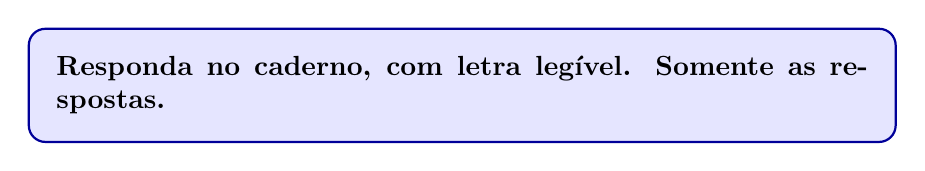
\begin{tikzpicture}
\node[rectangle, fill=blue!10, rounded corners=6pt, inner sep=10pt, draw=blue!60!black, thick]{
\begin{minipage}{0.85\linewidth}
\textbf{Responda no caderno, com letra legível. Somente as respostas.}
\end{minipage}
};
\end{tikzpicture}

\vspace{0.6cm}

\begin{enumerate}
\item O princípio fundamental da contagem diz que, quando um processo ocorre em etapas independentes, o número total de possibilidades é o produto das quantidades de escolhas de cada etapa. \textbf{Exemplo}: Para montar uma roupa, se tenho 3 camisetas e 2 calças, posso formar $3 \cdot 2 = 6$ combinações diferentes.

\item A \textbf{permutação} envolve todos os elementos e considera a ordem importante. Já o \textbf{arranjo} também considera a ordem, porém utiliza apenas parte dos elementos disponíveis.

\item A \textbf{combinação} deve ser usada quando a ordem dos elementos não faz diferença, ou seja, quando apenas o grupo formado é importante.

\item Um exemplo de situação com ordem relevante é escolher o 1º, 2º e 3º colocado de uma competição. A ordem dos colocados altera o resultado.

\item O fatorial aparece nas permutações porque a permutação de $n$ elementos é dada por $n!$, representando todas as maneiras diferentes de ordenar esses elementos.

\item Em sorteios e seleções, as combinações são usadas porque interessa apenas quem foi escolhido, não a ordem em que os escolhidos são selecionados.

\item A análise combinatória é importante porque ajuda a determinar o número de possíveis resultados, o que é essencial para calcular probabilidades e analisar dados estatísticos.

\item Escolher 3 representantes entre 10 alunos é um exemplo de \textbf{combinação}, pois apenas importa quem será escolhido, e não a ordem da escolha.
\end{enumerate}

\end{document}

